\chapter{Proceso de gestión}
\section{Estimaciones del proyecto}
Los recursos financieros de los que se disponen son limitados. Serán los participantes los que tendrán que invertir su dinero en el proyecto. Actualmente, se ha establecido un límite de 200 euros.\\

Como no poseemos datos estadísticos sobre los participantes del proyecto, se considerara la productividad de todos los participantes por igual. Así, la productividad del grupo será de 10 pm (personas mes). Considerando por lo tanto que 1 pm = 20 pd (personas día).\\

La estimación del coste del proyecto, se ha realizado conforme a horas de esfuerzo por persona.  Dando una productividad al alumno de un 67\%. Si el curso universitario consta de 270 días, entonces un estudiante puede ser capaz de aprovechar 180 días. Con un rendimiento medio al día de 1 hora, una persona tendrá una productividad de 180 horas. De esta forma, al ser 10 estudiantes universitarios se estima que costará 1800 horas. Para la planificación no se puede contar con el total de horas, puesto que no existe proyecto sin contratiempos. Por esta razón se ha considerado la regla del 80\%. Ésta dice, ``para poder obtener un coste real aproximado al coste esperado debemos planificar el 80\% del tiempo, puesto que el tiempo restante se invierte en imprevistos''.\\

En este proyecto tendremos dos peculiaridades añadidas que nos obligan a volver a aplicar dicha regla. El modelo de proceso usado (SCRUM) y el tipo de estrategia de desarrollo (desarrollo por prototipos). Esto lo tendremos en cuenta en la estimación, pero para que la planificación no se vuelva tríptica se añadirán como tareas estimadas los porcentajes de incertidumbre. Estimándose los imprevistos debidos a estas peculiaridades, quedando el tiempo a planificar en el 80\% del coste total, es decir, en 1440 horas. Porque, aunque es cierto que tendremos imprevistos, los prototipos nos aportan la reutilización de los mismos, abaratando costes y aumentando la productividad por hora invertida. 
  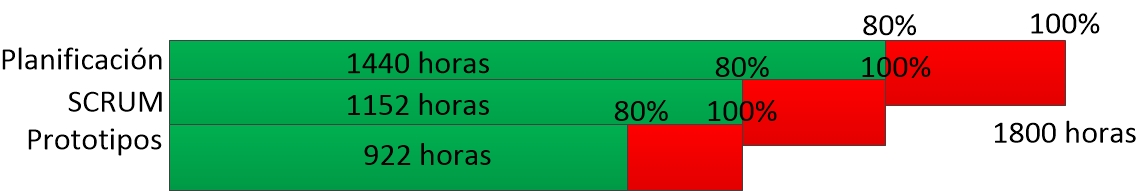
\includegraphics[width=0.96\textwidth]{2.GestionYPlanificacion/estimacion.jpg}

\section{Plan de proyecto}
\subsection{Módulos}
Los módulos tienen las funcionalidades agrupadas por prioridad. De esta forma los spint primero se centraran en las del módulo 1 y acabarán en el 3. Garantizando, que la aparición de algún riesgo afecte lo menos posible. También busca orientar la administración hacia el desarrollo software RUP, pretendiendo así el mejor seguimiento del proyecto por el profesor (cliente). Pudiendo asemejarse a funcionalidades por iteración.
\begin{itemize}

\item Módulo1
\begin{itemize}
\item	Control remoto de luces.
\item	Control de dispositivos por infrarrojos.
\item	Control remoto de la puerta del garaje.
\item	Control remoto de persianas.
\item	Aplicación IOS y Android.
\end{itemize}

\item Módulo2
\begin{itemize}
\item	Control remoto del telefonillo.
\item	Control de enchufe.
\item	Previsión meteorológica.
\item	Información de sensores meteorológicos.
\item	Información de sensores de movimiento.
\item	Aplicación web.
\end{itemize}

\item Módulo3
\begin{itemize}
\item	Perfiles de mandatos.
\item	Control remoto de Hardware.
\item	Modo offline.
\item	Control remoto de climatización.
\item	Recolección de datos sobre el uso de dispositivos.
\item	Monitorización consumo energético en tiempo real.
\end{itemize}

\end{itemize}
\subsection{Recursos del proyecto}
Los 10 componentes del grupo son: \\

Héctor Gutiérrez, Fernando Arturo Guzmán Almonte, Álvaro Morales Lozano, Luis Antonio Saavedra Palacios, Víctor Vicente, Miguel Alexander Maldonado Lenis, Alejandro Ladrón de Guevara, Víctor Ochoa Rodríguez, José Antonio Rey Álvarez, Colin Tirado Caamaño.\\

El calendario laboral asociado a cada uno de ellos es de 7 horas a la semana.\\
Los recursos materiales de los que se dispone son:
\begin{itemize}
\item	Arduinos	3
\item	Raspberry PI	1
\item	Protoboard	3
\item	Servidor	1
\item	Shield		2
\item	Conectores	2
\item	Maletines	1
\item	Entrenadores	*(libres en horario de clase facultad informática UCM)
\item	Soldadores	2
\end{itemize}
Todos ellos con disponibilidad total de horario salvo los entrenadores.

\subsection{Entregas}
Este proyecto tiene 2 entregas importantes:
\begin{itemize}
\item	22 enero. Se entregara toda la documentación y una demostración de un prototipo parcial de una funcionalidad básica.
\item	Mayo. Sera la entrega final del proyecto, que llevara un prototipo alpha estable del proyecto.
\end{itemize}

\subsection{EDT}
La estructura de descomposición del trabajo sigue el diagrama de la figura ~\ref{im:edt}

\begin{figure}[h]
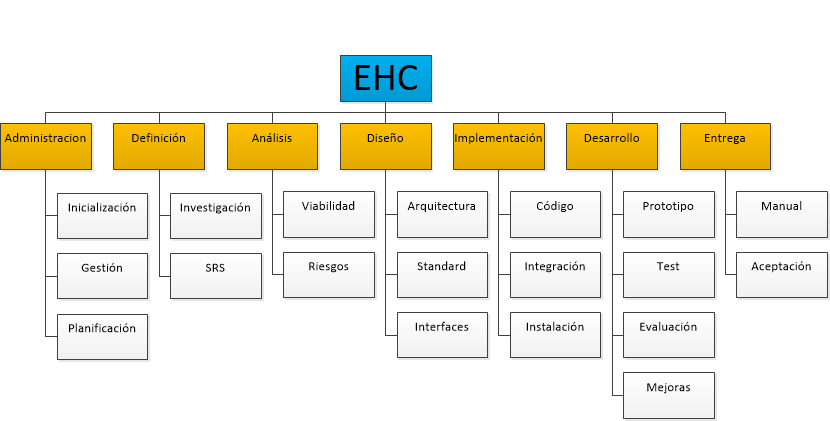
\includegraphics[width=0.9\textwidth]{2.GestionYPlanificacion/EDT.png}
\caption{Estructura de descomposición del trabajo}
\label{im:edt}
\end{figure}


Conforme a este, se han sacado las tareas de las funcionalidades definidas en los requisitos del proyecto. 
\section{Planificación del proyecto}
La planificación del proyecto se ha llevado a cabo utilizando una herramienta de gestión de proyectos llamada MS Project 2010. En él, se tienen todas las tareas asociadas a las funcionalidades que se quieren implementar. Puesto que no puede meterse en este documento, se adjunta un archivo llamado ``Microsoft Project - Plan de proyecto\_21enero.pdf'' con una captura de esta planificación.\\

Esa planificación, tiene desarrollada todas las tareas que se tendrán que hacer para ofrecer cierta funcionalidad. Pero éstas, se irán haciendo, conforme al sprint a los que pertenezcan. Dando nos la facilidad de elegir la tarea que más repercusión tenga (tarea critica) o la que más funcionalidad nos ofrezca (cuello de botella).
\section{Sprint }
Se ha decidido tener 3 sprint en el primer cuatrimestre, dirigidos a poder ofrecer un prototipo con funcionalidad infrarroja, en vistas a la primera entrega que será en enero.\\

Para el segundo cuatrimestre se espera poder hacer sprint más cortos, ya que no se desarrollara tanta documentación.
\section{Control y gestión del proyecto}
\subsection{Plan de gestión de requisitos}
Se prevé que los requisitos puedan cambiar, pero será fundamentalmente por mejoras en la fase de desarrollo, ligadas a la funcionalidad de los prototipos. Por lo que, más bien forma parte del desarrollo iterativo incremental.
\subsection{Plan de control de la planificación}
Al tener desarrolladas las tareas y estimas, el control del proyecto se lleva por cantidad de trabajo realizado, es decir esfuerzo realizado por unidad de tiempo. En nuestro caso esta relación será de 1 a 1 por simplicidad. Así podremos seguir la progresión del proyecto en un diagrama burn down que nos ofrece la herramienta CASE (MS Project 2010).
\subsection{Plan de control de calidad}
Para garantizar al cliente el correcto funcionamiento se tienen los test, que nos garantizaran su fiabilidad. Pero para garantizar la calidad del proyecto se tienen previstas como tareas ya consideradas (lanzadas en la planificación), revisiones técnicas formales sobre los diseños y las arquitecturas (no aparecen con ese nombre por especificar más la tarea). Que son la parte más críticas en hardware. Aunque estas se llevaran a cabo tras algún test, sea o no satisfactorio, puesto que no es tan fácil depurar hardware. \\

Al formar parte de la planificación, se puede decir que esas revisiones forman parte del proyecto, ya que se han contabilizado. Ofreciendo así una garantía de calidad mínima.
\section{Plan de gestión de riesgos}
Gracias a la detallada descomposición y a que estas sean tareas asequibles. Los riesgos asociados a índices catastróficos han desaparecido. Pero es cierto que podrían aparecer riesgos que también tengan repercusión notable sobre la funcionalidad, inicial tal y como se detalla en el documento de riesgos. La periódica actualización de la planificación nos avisara de la posible aparición, ofreciéndonos la posibilidad de tratar la mayor parte de ellos con anterioridad.
